\documentclass[xcolor=pdftex,dvipsnames,table]{beamer}
%
% Choose how your presentation looks.
%
% For more themes, color themes and font themes, see:
% http://deic.uab.es/~iblanes/beamer_gallery/index_by_theme.html
%
\mode<presentation>
{
  \usetheme{Szeged}    % or try Darmstadt, Madrid, Warsaw, ...
  \usecolortheme{dolphin} % or try albatross, beaver, crane, ...
  \usefonttheme{default}  % or try serif, structurebold, ...
  \setbeamertemplate{navigation symbols}{}  % uncomment to turn nav buttons off
  \setbeamertemplate{caption}[numbered]
  \setbeamercolor{framesource}{fg=gray}
  \setbeamerfont{framesource}{size=\tiny}
} 

\usepackage{amsmath}
\usepackage{comment}
\usepackage{geometry}
\usepackage{wrapfig}
\usepackage[english]{babel}
\usepackage[utf8x]{inputenc}
\usepackage[absolute,overlay]{textpos}
\usepackage{pgfpages}
\usepackage{parskip}
\usepackage{tcolorbox,fancyvrb,newverbs,xcolor,tikz}
\usepackage[thinlines]{easytable}

%%% Custom settings

\setbeameroption{hide notes} % Only slides
%\setbeameroption{show only notes} % Only notes
%\setbeameroption{show notes on second screen=right} % Both

\tcbuselibrary{skins,breakable}

% Give a slight yellow tint to the notes page
\setbeamertemplate{note page}{\pagecolor{yellow!5}\insertnote}\usepackage{palatino}

%%% Custom commands & environments

\newcommand{\source}[1]{
  \begin{textblock*}{8cm}(4.7cm,8.6cm)
      \begin{beamercolorbox}[ht=0.5cm,right]{framesource}
          \usebeamerfont{framesource}\usebeamercolor[fg]{framesource} Source: {#1}
      \end{beamercolorbox}
  \end{textblock*}
}

\newverbcommand{\cverb}{\color{teal}}{}

\newcommand*{\fvtextcolor}[2]{\textcolor{#1}{#2}}

\newenvironment{bgverbatim}[1]{
  \vspace{5pt}#1\VerbatimEnvironment
  \begin{tcolorbox}[breakable,spartan]% fontupper=\color{teal}
  \begin{Verbatim}[commandchars=&\[\]]}
  {\end{Verbatim}\end{tcolorbox}}

\newenvironment{wideitemize}{\itemize\addtolength{\itemsep}{5pt}}{\enditemize}

%%% Title page

\title[Generics and Sequences]{Kotlin - Generics and Sequences}
\author[Jacky Xu]{Jacky Xu}
\institute[RBC One Kotlin Study Group]{RBC One Kotlin Study Group}
\date{April 25, 2018}

\begin{document}

\begin{frame}
  \titlepage
\end{frame}

% Uncomment these lines for an automatically generated outline.
%\begin{frame}{Outline}
%  \tableofcontents
%\end{frame}

%%%%%%%%%%%%%%%%%%%%%%%%%%%%%%%%%%%%%%%%%%%%%%%%%%%%%%%%%%%%%%%%%%%%%%%%%%%%%%%%%%%%%%%%%%
\section{Generics Basics}
\stepcounter{subsection}

\begin{frame}[fragile]{Generics}
  \begin{wideitemize}
    \item Allows a class or function to operate on objects of various types
    \item Provides compile-time type safety
    \item Not much different from generics in Java
    \item Kotlin compiler can usually infer the parameterized type from the values provided
    \begin{bgverbatim}{\small}
val list1 = listOf(1, 2, 3)
val list2 = listOf("1", "2", "3")
    \end{bgverbatim}
  \end{wideitemize}
  
  \note[item]{Make sure there is internet connection.}
  \note[item]{Thank the audience for coming.}
\end{frame}

\begin{frame}[fragile]{Generics}
  \begin{wideitemize}
    \item Generic class:
    \begin{bgverbatim}{\small}
class Box<&fvtextcolor[red][T]>(val contents: List<&fvtextcolor[red][T]>)
    \end{bgverbatim}

    \item Generic function:
    \begin{bgverbatim}{\small}
fun <&fvtextcolor[red][T]> take(box: Box<&fvtextcolor[red][T]>) { ... }
    \end{bgverbatim}

    \item Generic interface:
    \begin{bgverbatim}{\small}
interface Formatter<&fvtextcolor[red][T]> { ... }
    \end{bgverbatim}
  \end{wideitemize}

  \note[item]{Show the GenericClass and GenericFunction code examples.}
\end{frame}

\begin{frame}[fragile]{Upper Bounds}
  \begin{wideitemize}
    \item We can specify upper bounds on type parameters
    \begin{bgverbatim}{\small}
// In Java:
class Box<T extends Fruit> { ... }

// In Kotlin:
class Box<&fvtextcolor[red][T: Fruit]>(val contents: List<T>)
    \end{bgverbatim}
  \end{wideitemize}
\end{frame}

\begin{frame}[fragile]{Upper Bounds}
  \begin{wideitemize}
    \item If there are multiple upper bounds, we must specify them by the \cverb|where| keyword:
    \begin{bgverbatim}{\small}
class Box<T>(val contents: List<T>) 
    &fvtextcolor[red][where T: Fruit, T: Round]
    \end{bgverbatim}

    \item A type parameter with no upper bound specified will have the upper bound of \cverb|Any?|
    \item Unlike in Java, there are no lower bounds in Kotlin
  \end{wideitemize}

  \note[item]{Even though there are no lower bounds, there are workarounds. 
    For example, we specify the type to be intravariant.}
\end{frame}

\begin{frame}[fragile]{Type Erasure}
  \begin{wideitemize}
    \item In Java, type information is lost at runtime to maintain backwards compatibility with previous versions of JVM.
    \item Since Kotlin runs on the JVM, its types are also erased.
  \end{wideitemize}
  \vspace{6pt}
  \begin{center}
    
\includegraphics[height=0.5\textheight,keepaspectratio]{images/type-erasure}
  \end{center}
\end{frame}

\begin{frame}[fragile]{Type Erasure}
  \begin{wideitemize}
    \item Kotlin compiler will try to infer type parameter at compile time:
    \begin{bgverbatim}{\small}
val strings = listOf("1", "2", "3")
println(strings is List<String>) // true
    \end{bgverbatim}

    \item If type parameter cannot be inferred at compile time, will throw compile time error:
    \begin{bgverbatim}{\small}
val anys = listOf("1", 2, 3.0)
println(anys is List<String>) // error
    \end{bgverbatim}
  \end{wideitemize}
\end{frame}

\begin{frame}[fragile]{Type Erasure}
  \begin{wideitemize}
    \item We can use \textbf{star projection} if we don't care about the type parameter:
    \begin{bgverbatim}{\small}
val anys = listOf("1", 2, 3.0)
println(anys is List<&fvtextcolor[red][*]>) // true
    \end{bgverbatim}
  \end{wideitemize}
\end{frame}

\begin{frame}[fragile]{Reified Types}
  \begin{wideitemize}
    \item Kotlin has a way of retaining type information at runtime, called \textbf{reification}
    \item Reification only works:
    \begin{itemize}
      \item In an \textbf{inlined function}
      \item If the generic type is preceded by the \cverb|reified| keyword
    \end{itemize}
    \begin{bgverbatim}{\footnotesize}
&fvtextcolor[red][inline] fun <&fvtextcolor[red][reified] T> hasType(box: Box<*>) =
    box.contents.any { it is T }
    \end{bgverbatim}
  \end{wideitemize}
\end{frame}

\begin{frame}[fragile]{Reified Types}
  \begin{wideitemize}
    \item How we \textbf{can} use reified type parameters:
    \begin{itemize}
      \item In type checks and casts (is, !is, as, as?)
      \item To use the Kotlin reflection APIs (::class)
      \item To get the corresponding java.lang.Class (::class.java)
      \item As a type argument to call other functions
    \end{itemize}
    \begin{bgverbatim}{\footnotesize}
inline fun <reified T> List<T>.printType() {
    println("This list contains elements " +
        "of type &textdollar{&fvtextcolor[red][T::class]}")
}
    \end{bgverbatim}
  \end{wideitemize}
\end{frame}

\begin{frame}[fragile]{Reified Types}
  \begin{wideitemize}
    \item How we \textbf{can't} use reified type parameters:
    \begin{itemize}
      \item Create new instances of the class specified as a type parameter
      \item Call methods on the companion object of the type parameter class
      \item Use a non-reified type parameter as a type argument when calling a function with a reified type parameter
      \item Mark type parameters of classes, properties, or non-inline functions as reified
    \end{itemize}
  \end{wideitemize}
\end{frame}

%%%%%%%%%%%%%%%%%%%%%%%%%%%%%%%%%%%%%%%%%%%%%%%%%%%%%%%%%%%%%%%%%%%%%%%%%%%%%%%%%%%%%%%%%%
\section{Variance}
\stepcounter{subsection}

\begin{frame}{Variance}
  \begin{wideitemize}
    \item Liskov Substitution Principle (LSP): A subtype can be substituted for its supertype without altering expected behavior.
  \end{wideitemize}
\end{frame}

\begin{frame}{Variance}
  \begin{center}
    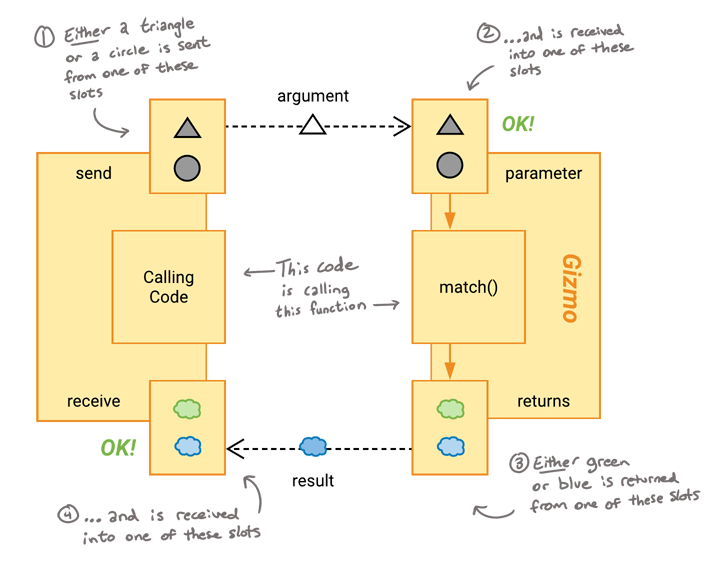
\includegraphics[height=0.9\textheight,keepaspectratio]{images/function-call-ok-annotated}
  \end{center}
  \source{https://typealias.com/guides/illustrated-guide-covariance-contravariance}
\end{frame}

\begin{frame}{Variance}
  \begin{center}
    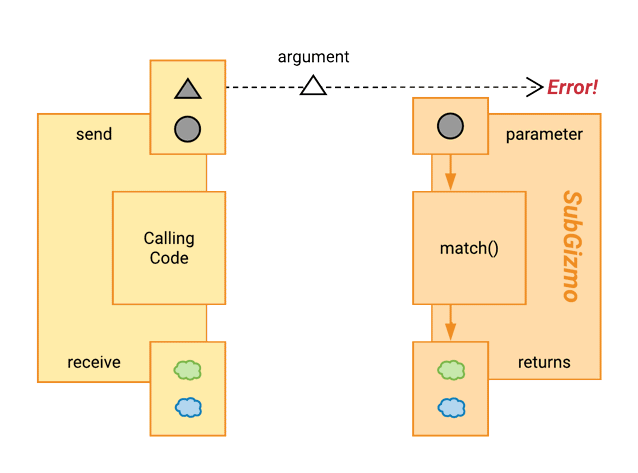
\includegraphics[height=0.9\textheight,keepaspectratio]{images/function-call-error-in}
  \end{center}
\end{frame}

\begin{frame}{Variance}
  \begin{center}
    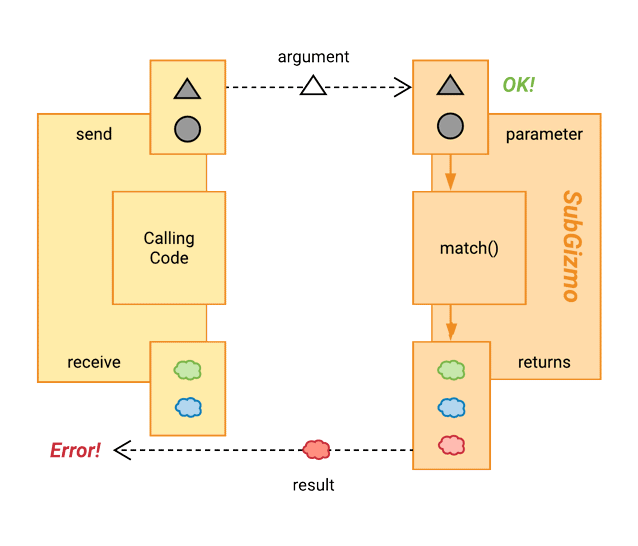
\includegraphics[height=0.9\textheight,keepaspectratio]{images/function-call-error-out}
  \end{center}
\end{frame}

\begin{frame}{Variance}
  \begin{center}
    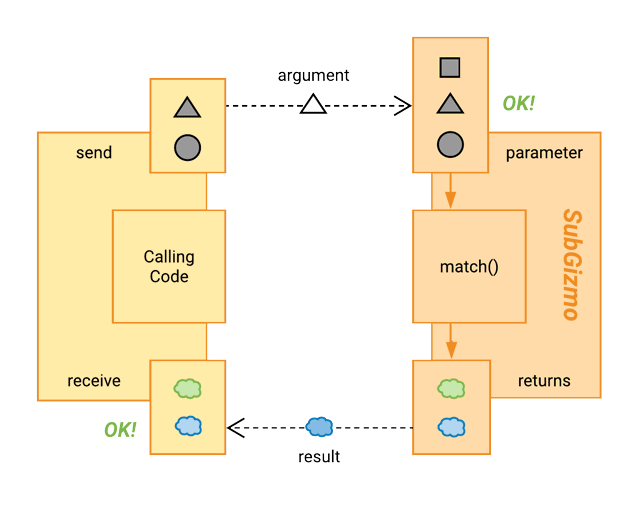
\includegraphics[height=0.9\textheight,keepaspectratio]{images/function-call-ok-contravariance}
  \end{center}
\end{frame}

\begin{frame}{Variance}
  \begin{center}
    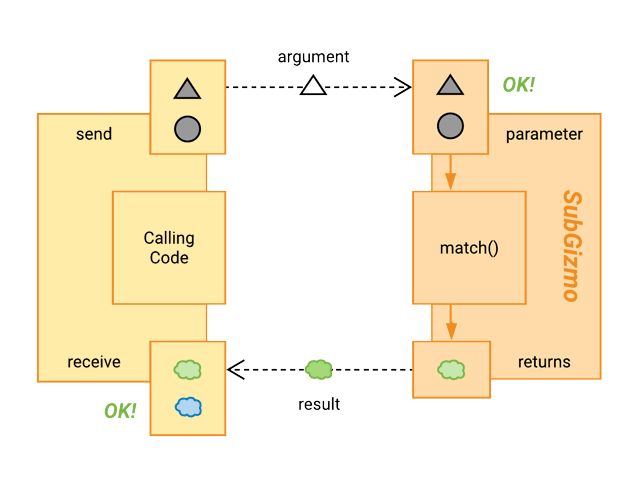
\includegraphics[height=0.9\textheight,keepaspectratio]{images/function-call-ok-covariance}
  \end{center}
\end{frame}

\begin{frame}{Rules of Variance}
  \begin{wideitemize}
    \item[1] A subtype must \textbf{accept at least} the same range of types as its supertype declares.
    \item[2] A subtype must \textbf{return at most} the same range of types as its supertype declares.
  \end{wideitemize}
\end{frame}

\begin{frame}{Covariance}
  \begin{wideitemize}
    \item A subtype must \textbf{return at most} the same range of types as its supertype declares.
    \item This relationship is called \textbf{covariance}
  \end{wideitemize}
  \begin{center}
    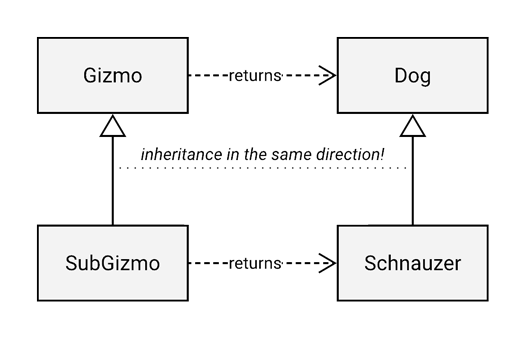
\includegraphics[height=0.5\textheight,keepaspectratio]{images/covariant-return-types}
  \end{center}
\end{frame}

\begin{frame}[fragile]{Covariance}
  \begin{wideitemize}
    \item We specify a type parameter of a class or interface to be \textbf{covariant} by prepending the \cverb|out| keyword.
    \item A contravariant type can only be used as a function return type; it can never be used as a function argument type (why?)
    \item A covariant type is said to be in the \textbf{out} position.
    \begin{bgverbatim}{\small}
data class Pair<&fvtextcolor[red][out] A, &fvtextcolor[red][out] B>(
    val first: A, val second: B)
fun <T> Pair<T, T>.toList(): List<T> 
    = listOf(first, second)
    \end{bgverbatim}
  \end{wideitemize}
\end{frame}

\begin{frame}{Contravariance}
  \begin{wideitemize}
    \item A subtype must \textbf{accept at least} the same range of types as its supertype declares.
    \item This relationship is called \textbf{contravariance}
  \end{wideitemize}
  \begin{center}
    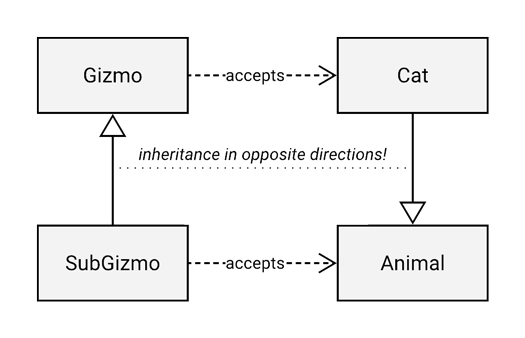
\includegraphics[height=0.5\textheight,keepaspectratio]{images/contravariant-argument-types}
  \end{center}
\end{frame}

\begin{frame}[fragile]{Contravariance}
  \begin{wideitemize}
    \item We specify a type parameter of a class or interface to be \textbf{contravariant} by prepending the \cverb|in| keyword.
    \item A contravariant type can only be used as function argument types; it can never be used as a function return type. (why?)
    \item A contravariant type is said to be in the \textbf{in} position.
    \begin{bgverbatim}{\small}
interface Comparable<&fvtextcolor[red][in] T> {
    operator fun compareTo(other: T): Int
}
    \end{bgverbatim}
  \end{wideitemize}
\end{frame}

\begin{frame}{Invariance}
  \begin{wideitemize}
    \item By default a type parameters are in neither the in nor the out position.
    \item An invariant type can be used in both function arguments and function return types.
    \item A covariant type cannot be the type of a var property in a primary constructor of a class.
    \item A contravariant type cannot be the type of any property in a primary constructor of a class.
  \end{wideitemize}
\end{frame}

\begin{frame}[fragile]{Type Projection}
  \begin{wideitemize}
    \item All of the variance described above with the 'in' and 'out' keywords is called \textbf{declaration-site variance}
    \item In Kotlin we can also use \textbf{use-site variance}, also called \textbf{type projection}
    \item When the \cverb|in| or \cverb|out| keyword is specified in a function declaration, then the type passed in is treated as if it were contravariant or covariant, respectively.
  \end{wideitemize}
  \begin{center}
    \hspace{-1cm}
    \begin{TAB}(r,0.5cm,0.5cm)[4pt]{|ccc|}{|c|c|}% (rows,min,max)[tabcolsep]{columns}{rows}
      \verb|? super T| & \verb|<==>| & \verb|in T| \\
      \verb|? extends T| & \verb|<==>| & \verb|out T|
    \end{TAB}
  \end{center}

  \note[item]{Use site variance is closer to how Java handle variance, whereas declaration site variance is more of a Kotlin thing.}
\end{frame}

%%%%%%%%%%%%%%%%%%%%%%%%%%%%%%%%%%%%%%%%%%%%%%%%%%%%%%%%%%%%%%%%%%%%%%%%%%%%%%%%%%%%%%%%%%
\section{Sequences}
\stepcounter{subsection}

\begin{frame}[fragile]{Sequences}
  \begin{wideitemize}
    \item A \textbf{sequence} in Kotlin is pretty much the same as a stream in Java 8.
    \item Kotlin re-implemented this because Java streams aren't available in every platform. 
    \begin{itemize}
      \item On Android in the past, Java 8 is not fully supported.
    \end{itemize}
    \item Sequences have a greater range of supported operations than Java streams and are less verbose.
    \begin{itemize}
      \item Eg. filterIsInstance(), zip(), and associate()
    \end{itemize}
    \item We can perform all stream operations on any collection without converting them to a stream first.
  \end{wideitemize}
\end{frame}

\begin{frame}[fragile]{Using Sequences}
  \begin{wideitemize}
    \item As with streams, sequences are evaluated \textbf{lazily}, whereas collections are evaluated \textbf{eagerly}.
    \item Two types of operations:
    \begin{itemize}
      \item \textbf{Intermediate operation}: returns another sequence, which is produced lazily.
      \item \textbf{Terminal operation}: returns a concrete collection or value, and evaluates all operations previously defined in an optimized manner.
    \end{itemize}
    \item Unlike in Java, sequences can be iterated multiple times (unless specified in the docs).
    \begin{itemize}
      \item We can constrain a sequence to be only iterable once with \cverb|constrainOnce()|.
    \end{itemize}
  \end{wideitemize}
\end{frame}

\begin{frame}[fragile]{Using Sequences}
  \begin{wideitemize}
    \item When we \textbf{should} use sequences:
    \begin{itemize}
      \item When dealing with large collections with many operations.
      \item When the number of items is infinite or unknown.
      \item When processing a large number of items with some filtering operation. (eg. first\{\} or last\{\})
    \end{itemize}
    \item When we \textbf{should not} use sequences:
    \begin{itemize}
      \item When dealing with small collections.
      \item When passing/returning the intermediate results to functions.
      \item When you need to access only the nth item.
    \end{itemize}
  \end{wideitemize}

  \note[item]{"When dealing with large collections" - it avoids the creation of intermediate collections that happens when we just use stream operations on a normal collection without turning it into a stream first.}
  \note[item]{Since collections now have stream operations defined on them, readability is not an advantage for using streams.}
  \note[item]{"When we need to store intermediate results. Use a collection instead." - if we store the intermediate results in a sequence, all consumers using this sequence will have to re-compute all operations again.}
\end{frame}

\begin{frame}[fragile]{Using Sequences}
  \begin{center}
    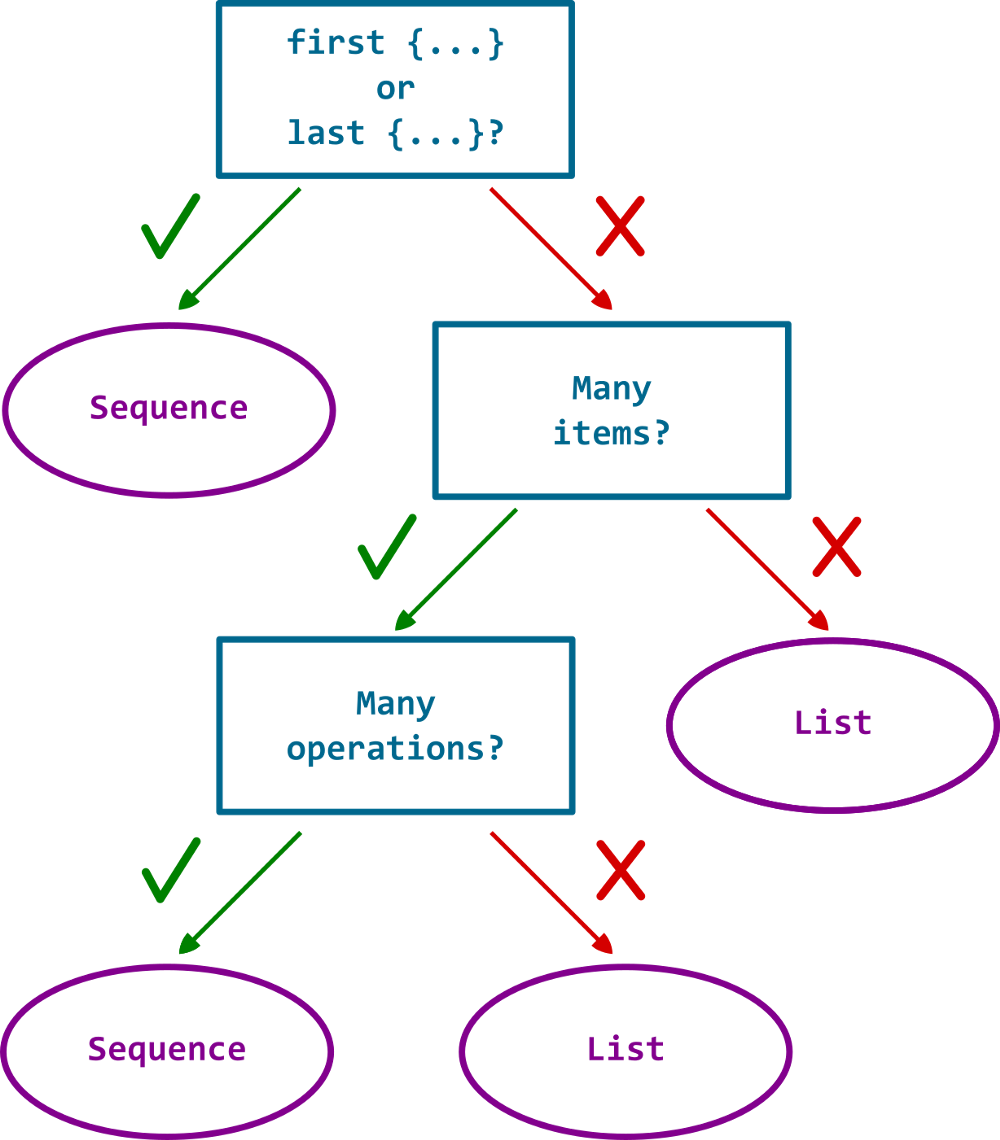
\includegraphics[height=0.75\textheight,keepaspectratio]{images/sequences-decision-tree}
  \end{center}
  \source{https://proandroiddev.com/sequences-a-pragmatic-approach-9d4296086a9d}
\end{frame}

\begin{frame}[fragile]{Creating Sequences}
  \begin{wideitemize}
    \item Any iterable can be converted to a sequence using the \cverb|asSequence()| method.
    \item The \cverb|generateSequence()| function and its variants which are helpers for creating sequences.
    \item The \cverb|buildSequence()| function can be used to yield values in the sequence, similar to how Typescript's generators are implemented.
    \begin{itemize}
      \item This feature is experimental.
    \end{itemize}
    \begin{bgverbatim}{\small}
val naturalNumbers: Sequence<Int> 
    = &fvtextcolor[red][generateSequence](0) {it + 1}
    \end{bgverbatim}
  \end{wideitemize}
\end{frame}

%%%%%%%%%%%%%%%%%%%%%%%%%%%%%%%%%%%%%%%%%%%%%%%%%%%%%%%%%%%%%%%%%%%%%%%%%%%%%%%%%%%%%%%%%%
\section{Conclusion}
\stepcounter{subsection}

\begin{frame}[fragile]{Resources}
  \begin{wideitemize}
    \item Assignment: Udemy's Kotlin challenges (Round Five)
    \item Additional problems are in the git repository of this session, under the \verb|com.rbc.rbcone.studygroup.kotlin| package.
    \begin{itemize}
      \item Six problems total.
      \item Solutions are in the \verb|solutions| branch.
    \end{itemize}
    \item Slides and code examples are in the git repository.
  \end{wideitemize}
\end{frame}

\begin{frame}[fragile]{Conclusion}
  \centering
  \vspace{25pt} 
  \LARGE
  \emph{Thank you}
  \small
  \vspace{5pt}
  \begin{center}
    
\includegraphics[height=0.5\textheight,keepaspectratio]{images/cup-of-t}
  \end{center}
\end{frame}

%%%%%%%%%%%%%%%%%%%%%%%%%%%%%%%%%%%%%%%%%%%%%%%%%%%%%%%%%%%%%%%%%%%%%%%%%%%%%%%%%%%%%%%%%%
\end{document}

